% Chapter Template

\chapter{Data gathering and preprocessing} % Main chapter title

\label{Chapter2} % Change X to a consecutive number; for referencing this chapter elsewhere, use \ref{ChapterX}

%----------------------------------------------------------------------------------------
%	SECTION 1
%----------------------------------------------------------------------------------------

Data was sourced from several streams. The Icelandic Meterological Office (IMO) provided measurements from weather stations all around the Iceland. NWP data was downloaded from Copernicus Arctic Regional Reanalysis dataset (CARRA). A land elevation model was also provided by IMO.

\section{Automatic Weather Station Data}

IMO provided 10 minute measurements from \nStationsMin weather stations all around Iceland. The measurements that met the filtering criteria, started in \startDateVedur and ended in 2023 (the year measurements were provided). Of these \nStationsMin stations, \nVedurMin were from IMO Íslands and placed at 10 meters above ground, while the rest (\nVGMin) were from \href{https://www.vegagerdin.is/}{the Icelandic Road and Coastal Administration (IRCA)} and placed at 6-7 meters above ground\cite{vegagerdin_postur}. The location of these weather stations can be seen in Figure \ref{fig:aws_map}. The information that is provided by these Automatic Weather Stations (AWS) is presented in two different type of data files, hourly and 10 minute files. The hourly files are summations of the 10 minute files, with the exception that errors, such as nails, still in the 10 minute files should have been removed from the hourly documents. Nails, are sharp increases from the rest of the data and are unrealistic outliers that are considered measurement errors and are discarded. Each type of document contain the following information: the date and time, the station number (that can be converted to the coordinates using another data set), the average wind speed ($f$), the wind gust ($f_g$), the standard deviation of the wind gust, the direction of the wind ($d$) and the standard deviation for the wind direction. These measurement started at the end of the 20th century, when the first AWS stations was installed. More have been added in the following decades. This thesis does not look at the data as a time series, it tries to make predictions using only the information at a given point in time.

\begin{figure}
    \centering
    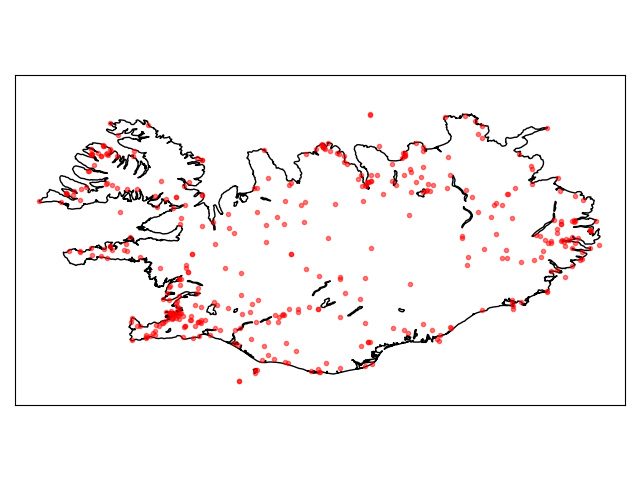
\includegraphics[scale = 0.75]{Figures/weather_stations_2024-04-09.png}
    \caption[Locations of automatic weather stations in Iceland]{Locations of all 412 stations that were looked at in this study. Most of these were from IMO but over a hundred were from IRCA. IMO AWS are placed at 10 meters above ground, while IRCA stations are placed at around 6-7 meters above ground.}
    \label{fig:aws_map}
\end{figure}

These 10 minute measurements were filtered to only include measurements where the average wind speed was at or above \averageWindSpeedLimit m/s. They were also filtered in such a way that only the highest value in any given 48 hour span is considered. This can be seen in Code Listing \ref{code:filter48hr}. Any measurement that is within a 48 hour interval centered on of the current highest is removed. This is done for each station and iteratively until all measurements have been removed.

\begin{lstlisting}[style = Python, caption = {[Filter points over 48 hour interval] Filter all measured points so to only keep the highest value in any 48 hour interval for a given station. For a given station, the highest wind speed recorded is selected. Then any measurement in a 48 hour interval, centered on the highest wind speed, for that given station, is removed. This is then done iteratively until we are left with an empty dataframe.}, label = code:filter48hr]
    for station in tqdm(stations, total = len(stations)):
        subset_df = vedur_df[station == vedur_df.stod]
        subset_df = subset_df.reset_index(drop = True)

        while not subset_df.empty:
            idx = subset_df.f.idxmax()
            time_of_max = subset_df.iloc[idx].timi

            filtered_data.append(subset_df.iloc[idx])

            subset_df = subset_df[abs(subset_df.timi 
                - time_of_max) >= pd.Timedelta(threshold)]

            subset_df = subset_df.reset_index(drop = True)  
\end{lstlisting}

When these two filterings have been done, the end result is \nStationsMin stations that meet these criteria. Of these, \nVedurMin belong to IMO and \nVGMin belong to IRCA. The number of observations by year can be seen in Figure \ref{fig:occurrences_by_year}. The first observations occurring in \startDateVedur and the latest in 2023.

\begin{figure}
    \begin{center}
        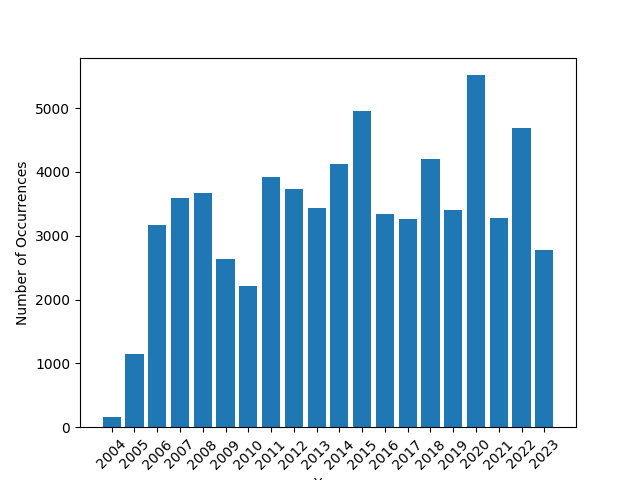
\includegraphics[scale = 0.75]{Figures/occurrences_by_year.png}
    \end{center}
    \caption[Measurements that fit filtering by year (from \startDateVedur to 2023).]{The total number of measurements by year after filtering by average wind speed limit of \averageWindSpeedLimit m/s and clearing the neighborhood using filtering method described in code listing. The measurements provided were sparse for years before 2005, as can be seen for 2004. Years before 2005 will thus be ignored.}
    \label{fig:occurrences_by_year}
\end{figure}

Looking at the number of measurements that meet these criteria for a given station, Figure \ref{fig:occurrences_by_station_20} shows only one station has over 1000 measurements that fit the criterias.

\begin{figure}
    \centering
    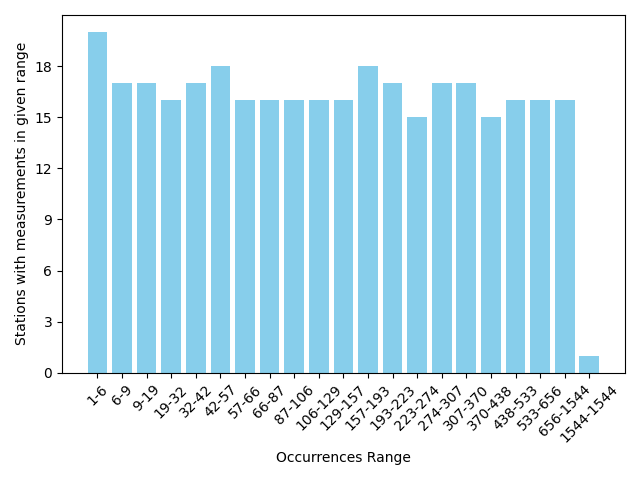
\includegraphics[scale = 0.75]{Figures/station_occurrences_20.png}
    \caption[Number of stations that have measurements in a range.]{The number of stations that have a-b measurements represented in filtered data. That is station x may have c measurements represented and $\protect a <= c < b$. Station x will then add to the count of column labeled $\protect [a, b[$.}
    \label{fig:occurrences_by_station_20}
\end{figure}

\section{CARRA Data}
    The CARRA dataset goes back to September 1991 and is currently updated monthly, with a latency of 2-3 months\cite{carra_information}. The oldest IMO data point that fulfills given criteria is from \startDateVedur. This is covered by CARRA. A few of the newer points from AWS were not available from CARRA when data was gathered. The CARRA dataset is available for two regions, west and east. Each of these covers a vastly larger area than the area of interest. This leads to having to store a large amount of data, because it is not possible to ask for specific points of interest. To get the data one has two options. Their web interface or using their API client. Using the API client is the only realistic option here, as there were thousands of requests made for different times.

Each request is made by going through all instances of the IMO data after filtering (by mean wind speed reaching \averageWindSpeedLimit m/s over a 10 minute interval). For each such observation in the IMO data, two API calls excluding redundancy are needed. One for the 3 hour interval before and one for the 3 hour interval after, if the data point doesn't fall exactly on one of the three hour interval times. That is if the observation was at 13:00, CARRA data for noon and 15:00 would have to be queried. Date and times were generated automatically from the AWS and requested by calling the client. Using these datapoints, interpolation was used to get an estimation for the point of the given weather station. The CARRA data contains several types of layers. These are single levels, model levels, height levels, pressure levels. The data for this observation was downloaded from height levels. That is, data was requested at heights of 15, 150, 250 and 500 meters above ground. For each point 4 parameters were requested, wind speed, wind direction, pressure and temperature. Each of these features needed to be interpolated to create data for model to be trained on.

After using this method to request terabytes of data, it was discovered that it was possible to query a specific area. This decreased the size of each file from around 50 MB to around 2 MB. The bottleneck for retrieving the data is the request time. The time the request is queued and running (server preparing the data) before it began downloading. This could range from almost immediate to 30 minutes. This problem was exacerbated by the fact that the climate data store (CDS) was undergoing updates during \href{https://forum.ecmwf.int/t/a-new-cds-soon-to-be-launched-expect-some-disruptions/1607}{the winter and spring of 2023/2024}, which increased the wait time and sometimes resulted in queries not being responded to. This meant that the time it would take to retrieve the remaining information went from around a day, when the requests were at their quickest, to many months, something that would not be possible given the time frame of the project. Fortunately these problems were only particularly time consuming during mid winter.

\subsection{Statistical Analysis of Measurements}
The data gathered from AWS showed inconsistencies due to significant gaps in data coverage in the early 2000s and 90s. This is shown in Figure \ref{fig:measurements_by_year}. It is important to note that Figure \ref{fig:measurements_by_year} and subsequent figures show number of measurements in logarithmic scale. Late in the process of making this thesis, it was discovered that data was missing. Most data points before 2005 had not been provided. Eventually this missing data was provided but the decision was made to exclude that data due to time constraints. Using only data from 2005 to 2023, means that all years cover the entire year. Thus the data was filtered to only include these years. For some reason there were a hundred or so measurements from 1990.

\begin{figure}
    \centering
    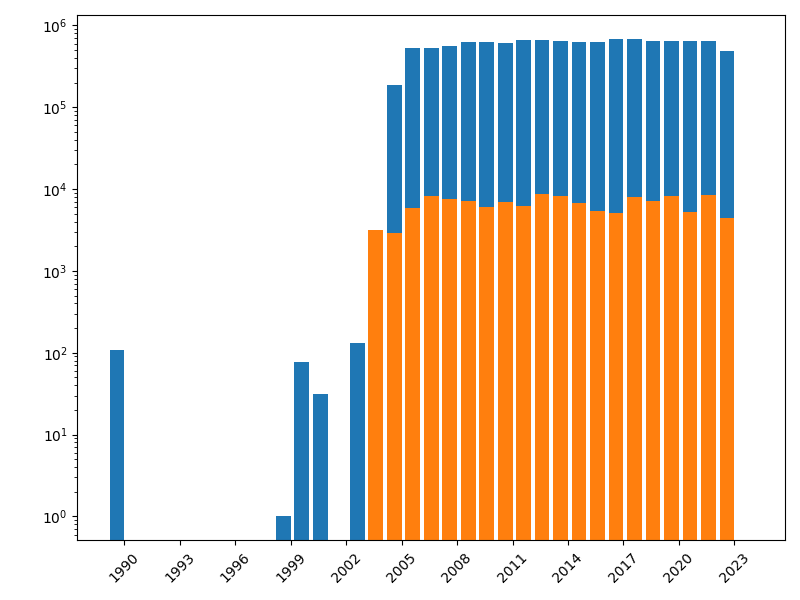
\includegraphics[scale = 0.75]{Figures/measurements_by_year.png}
    \caption[Number of measurement data points by year.] {Number of measurement data points by year. The effect of filtering by average windspeed limit shown in the orange overlay. It is important to note that the y-axis scale is logarithmic. If this was not the case, then the filtered values would not be clearly displayed.}
    \label{fig:measurements_by_year}
\end{figure}

It is a good sanity check to look at figures like Figure \ref{fig:measurements_by_year}. If there were massive discrepancies by year, then some data is missing. Another way to look at the distribution of measurement over time is to look at it by month, as in Figure \ref{fig:measurements_by_month}. The total measurements is evenly distributed over the months. As expected higher winds occur during the winter months, with only a few hundred wind measurements reaching \averageWindSpeedLimit.

\begin{figure}
    \centering
    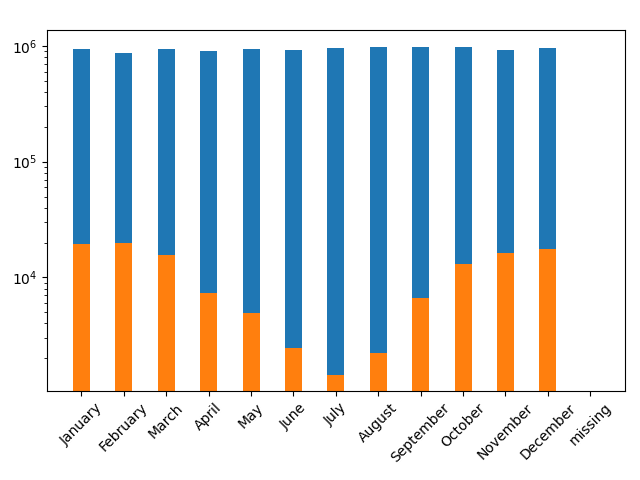
\includegraphics[scale = 0.75]{Figures/measurements_by_month.png}
    \caption[Number of measurement data points by month.]{Number of measurement data points by month. The effect of filtering by average windspeed limit shown in the orange overlay. This filtering shows us what we would expect to see. We can see that we have fewer extreme wind speeds during summer as compared to winter.}
    \label{fig:measurements_by_month}
\end{figure}

Another thing to look at is the number of average wind speed measurements by interval wind speed interval. This is shown in Figure \ref{fig:measurements_by_windspeed}. This figure shows the expected, the number of measurements at higher wind speeds decrease. The orange overlay shows the section that is considered in this thesis.

\begin{figure}
    \centering
    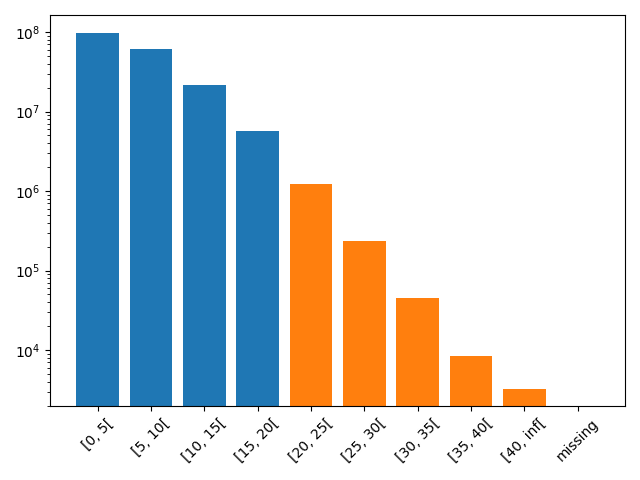
\includegraphics[scale = 0.75]{Figures/measurements_by_windspeed.png}
    \caption[Number of measurement data points by wind speed.]{Number of measurement data points by wind speed. The effect of filtering by average windspeed limit shown in the orange overlay. The filtering obviously just selects the columns to the right and including column $\protect [20, 25[$.}
    \label{fig:measurements_by_windspeed}
\end{figure}

Looking at Figure \ref{fig:measurements_by_windgust} something strange seems to be happening. The orange overlay shows the number of gust values where the wind speed is over \averageWindSpeedLimit m/s and some of the gust values is lower than that. This shows the relevancy of looking at such figures. These data points, where the average wind speed is higher than the gust speed, are filtered out later in the preprocessing pipeline. Note that there are seemingly no missing values for wind speed, wind gust and wind direction, but there is missing standard deviations for these parameters.

\begin{figure}
    \centering
    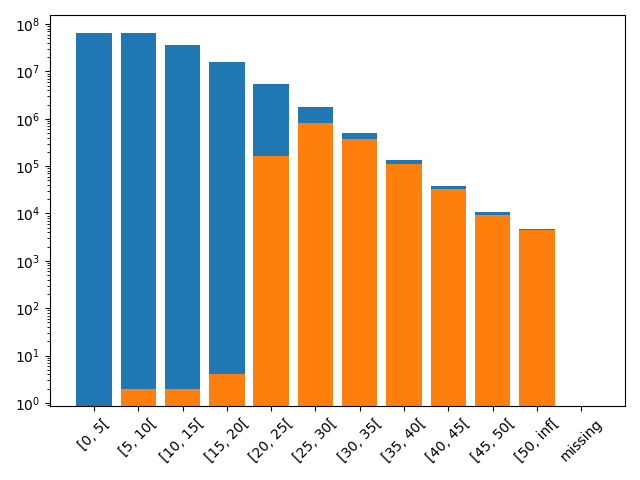
\includegraphics[scale = 0.75]{Figures/measurements_by_windgust.png}
    \caption[Number of measurement data points by wind gust.]{Number of measurement data points by wind gust. The effect of filtering by average wind speed limit shown in the orange overlay. Here we might expect to see some discrepancies in the columns. That is, the orange overlays should not completely cover all columns. This is because we select by windspeed and not gust. There should be no coverage below the average wind speed limit of \averageWindSpeedLimit m/s.}
    \label{fig:measurements_by_windgust}
\end{figure}


\section{Elevation data}
IMO provided a TIFF file containing the elevation of Iceland on a 20 meter by 20 meter grid. This file encompasses Iceland and is around 685 MB. A good amount of time was spent finding a data structure that was best for lookup when trying to find points within a certain area. The country was divided into 10 parts (as only around 13\% of the file was able to be read into memory at each time as a part of dictionary object) with boundary boxes. The Python package Rasterio allowed for quick lookup with it's index and the affine transform. Using this package it is possible to quickly look up elevation given coordinates using matrix calculations.